\Chapter{Introduction}
%%%%%%%%%%%%%%%%%%%%%%%%%%%%%%%%%%%%%%%%%%%%%%%%%%%%%%%%%%%%%%%%%%%%%%%%%%%%%%%%%%%%%%%%%%%%
%%%%%%%%%%%%%%%%%%%%%%%%%%%%%%%%%%%%%%%%%%%%%%%%%%%%%%%%%%%%%%%%%%%%%%%%%%%%%%%%%%%%%%%%%%%%
\Section{Motivation} \label{sec:motivation}
%%%%%%%%%%%%%%%%%%%%%%%%%%%%%%%%%%%%%%%%%%%%%%%%%%%%%%%%%%%%%%%%%%%%%%%%%%%%%%%%%%%%%%%%%%%%
%%%%%%%%%%%%%%%%%%%%%%%%%%%%%%%%%%%%%%%%%%%%%%%%%%%%%%%%%%%%%%%%%%%%%%%%%%%%%%%%%%%%%%%%%%%%

A new generation of accelerators dedicated to High Energy Physics
(HEP), would likely be of the TeV scale. Reduction in the size and cost
of such machines is key to their feasibility. 
Investigation into a high gradient candidates for future HEP machines is an active research. 
Traditional accelerating gradients are on the order of 10's of MV/m
with the power source being a klystron gallery.
High gradient structures and schemes such as the 
short pulse, two-beam acceleration (TBA) scheme 
at the Argonne Wakefield Accelerator (AWA) facility
use novel structures to reach 100's of MV/m or more. 
A goal of the AWA group is to demonstrate fully staged TBA, 
achieving a gradient of 250 MV/m. If successful, this would
be the only facility in the world capable of such gradients used for
acceleration of a beam.

TBA requires a drive beam to pass through a decelerating structure and
lose energy through wakefield generation. The electromagnetic wake
is coupled from the decelerator into an accelerating structure, where
the electric field is used to accelerate a second beam. 
This requires two complete and separate beamlines 
operating synchronously with each other.  
The wakefield structures can be metallic or dielectric on either beam line. 
Dielectric structures, having no irises, are simple to manufacture and have demonstrated
high gradient capability at \SI{100}{MV/m} \cite{WeiPaper}. 

The Compact Linear Collider (CLIC) collaboration, proposes a similar TBA scheme with
a \SI{240}{ns} pulse design. This limits the acceleration gradient
to roughly \SI{150}{MV/m} at room temperature due to rf breakdown \cite{CLICdesignReport}.
Higher gradients could be reached when driven by a very short drive
beam pulse, such as the \SI{20}{ns} pulse length proposed by AWA \cite{WeiPaper}. 
While the peak power and gradients are considerably larger in the short pulse scheme, 
the average power is still feasible and within current technology capabilities.
While the two groups vary on approach, they agree that TBA would 
require less infrastructure when constructing a linear TeV scale machine, 
versus the cost of more conventional technology. 

For example, a case study was done comparing the infrastructure 
needed when using traditional \SI{50}{MW} klystron sources.
It would take roughly 35,000 klystrons to construct a linear machine to deliver the same 
\SI{9.2}{TW} power required in the CLIC design specification reports \cite{CLICdesignReport}. 
With TBA, CLIC projected a \SI{3}{TeV} energy at a length of \SI{48}{km}.
In contrast, the Next Linear Collider (NLC) collaboration projected a \SI{1}{TeV} machine 
with length \SI{26}{km}, using X-band klystrons \cite{NLC}. 
This drastic difference occurs in the infrastructure needed to generate and transfer
RF power in the two cases. In TBA, a high charge bunch train is generated in 
a photoinjector and propagated down stream using conventional technology 
(accelerating structures, quads, dipoles, etc). After it has reached the design energy
is focused into specially designed wakefield structures (decelerating structure).
The RF is then generated in the decelerating structure and supplied to the witness 
beam line through a waveguide connection. This has two benefits over traditional klystron technology.
One, you can have structures at higher frequencies (any multiple of the machine frequency), 
which helps push the gradient. Readily available and production klystrons are limited in this aspect.
Second, all the waveguide infrastructure needed to connect a klystron to the accelerating 
structures is eliminated. There is the initial cost near the photoinjector, 
but downstream, much of the infrastructure costs are eliminated.
Theoretically, TBA can deliver the same amount of power as conventional methods with less 
infrastructure, and therefore lower cost, in the case of a large machine. 

Before a detailed understanding of the power and infrastructure trade offs 
can be obtained, the feasibility of staged TBA must be be demonstrated.
Demonstration of staging is especially important, 
as no high energy machine can be built without staging.
Staging is the ability to use two successive accelerating modules to synchronously accelerate 
the same particle bunch. While simple in principle, the difficulties 
in achieving staging should not be underestimated. 
Demonstration of staging proves that a TBA scheme can be scaled to high energies, and whether it is 
feasible to use such methods. Single stage TBA, and staging 
in a simplified scheme have been demonstrated at the AWA in 2016 \cite{tba2017}.
In the simplified scheme, both bunch trains travel through two decelerating stages.
This causes energy loss in stage 1 as the the second bunch train travels to stage 2.
\begin{figure}
	\begin{center}
		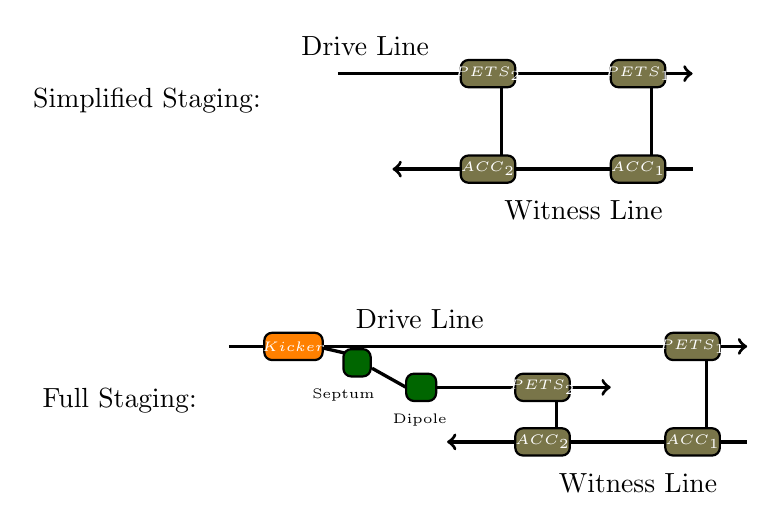
\begin{tikzpicture}[scale=\textwidth/35cm, text=black]
		\def \gunleft {-1.0}
\def \gunright {0.3}
\def \loneright {1.0}
\def \ltworight {2.0}
\def \lthreeright {3.0}
\def \lfourright {4.0}
\def \lfiveright {5.0}
\def \lsixright {6.0}
\def \quadone {7.3}
\def \quadfour{16}

%Full Staging
\draw[very thick, ->] (8,1) -- (27,1);

%Line between kicker and septum
\node[] at (15,2) {Drive Line};
\node[] at (23,-4) {Witness Line};
\draw[very thick] (\lsixright+5.2,1.0) -- (12.5,0.7);

%Kicker 
\draw[fill=orange,  thick, rounded corners =0.1cm] (\lsixright+3.3,0.5)rectangle ({\lsixright+0.84+4.6},1.5) node[pos=.5, white] {\tiny $Kicker$};
%Septum
\node[] at (12.2,-0.8) {\tiny Septum};
\draw[fill=black!60!green,  thick, rounded corners =0.1cm] (12.2,0.9)rectangle ({13.2},-0.1) node[pos=.5, white] {};
%Line between kicker and septum
\draw[very thick] (13.25,0.2) -- (14.5,-0.5);
%Dipole
\node[] at (15,-1.7) {\tiny Dipole};
\draw[fill=black!60!green, thick, rounded corners =0.1cm] (14.5,0.0)rectangle ({15.6},-1.0) node[pos=.5, white] {};
%Line between dipole and quads
\draw[very thick, ->] (15.6,-0.5) -- (22,-0.5);
%Witness
\draw[very thick, <-] (16,-2.5) -- (27,-2.5);
%Waveguide
\draw[very thick] (20,-0.5) -- (20,-3);
%Waveguide
\draw[very thick] (25.5,1.5) -- (25.5,-3);
%PETS2
\draw[fill=black!60!yellow,  thick, rounded corners =0.1cm] (18.5,0.0)rectangle (20.5,-1) node[pos=.5, white] {\tiny$\text{PETS}_2$};
%PETS1
\draw[fill=black!60!yellow,  thick, rounded corners =0.1cm] (24,1.5)rectangle (26,0.5) node[pos=.5, white] {\tiny$\text{PETS}_1$};
%ACC2
\draw[fill=black!60!yellow,  thick, rounded corners =0.1cm] (18.5,-2)rectangle (20.5,-3) node[pos=.5, white] {\tiny$\text{ACC}_2$};
%ACC1
\draw[fill=black!60!yellow,  thick, rounded corners =0.1cm] (24,-2)rectangle (26,-3) node[pos=.5, white] {\tiny$\text{ACC}_1$};



%Simplified Staging



\draw[very thick, ->] (12,11) -- (25,11);

%Line between kicker and septum
\node[] at (13,12) {Drive Line};
\node[] at (21,6) {Witness Line};

%Witness
\draw[very thick, <-] (14,10-2.5) -- (25,10-2.5);
%Waveguide
\draw[very thick] (18,11.5) -- (18,7);
%Waveguide
\draw[very thick] (23.5,11.5) -- (23.5,10-3);
%PETS2
\draw[fill=black!60!yellow,  thick, rounded corners =0.1cm] (16.5,11.5)rectangle (18.5,10.5) node[pos=.5, white] {\tiny$\text{PETS}_2$};
%PETS1
\draw[fill=black!60!yellow,  thick, rounded corners =0.1cm] (22,11.5)rectangle (24,10.5) node[pos=.5, white] {\tiny$\text{PETS}_1$};
%ACC2
\draw[fill=black!60!yellow,  thick, rounded corners =0.1cm] (16.5,8)rectangle (18.5,7) node[pos=.5, white] {\tiny$\text{ACC}_2$};
%ACC1
\draw[fill=black!60!yellow,  thick, rounded corners =0.1cm] (22,8)rectangle (24,7) node[pos=.5, white] {\tiny$\text{ACC}_1$};








		\node[fill=white, inner sep=2pt] (txt2) at (5,10) {Simplified Staging:};
		\node[fill=white, inner sep=2pt] (txt2) at (4,-1) {Full Staging:};
		\end{tikzpicture}
	\end{center}
	\caption{Simplified drawing of the two staging schemes.
		The arrows indicate what direction the beams travels.
		'Simplified staging' refers to experiments that took place at the AWA  prior to 2017.
		'Full Staging' refers to the TBA scheme that is the subject of this thesis.
		Installation efforts are currently ongoing.
		PETS stands for Power Extraction and Transfer Structure, and ACC stands for Accelerating structure. 
		The subscript on each structure refers to which stage the structures belong to (first or second). 
		In the simplified staging scheme the stages are not separated, meaning bunch train two travels
		through and loses energy in the first stage before reaching the second stage.
		This is prevented by separate beam lines in the full staging layout. }
	\label{fig:one}
\end{figure}

Fully staged TBA introduces a fast rise time kicker
and subsequent dogleg-like beam line. In this scenario, bunch trains can be 
be directed to two independent decelerating structures. 
Therefore you can extract the maximum amount of power in each stage.
The thesis work included experimental preparation of fully staged TBA, 
along with beam line design and optimization. 

Chapter 2 details the experimental setup, which included ultraviolet laser pulse train improvement, 
which improves the RF power generation in the wakefield structures.
Also discussed are measurements of the RF power in the gun and linac cavities.
Description of beam size analysis and an image processing script written in Python is covered.
In Chapter 3, the simulation code, OPAL~\cite{opal}, and model used for beam line design is covered in detail.
Benchmarking and initial optimization work is discussed. The photoinjector was optimized for \SI{40}{nC}. 
In Chapter 4, the design of a stripline kicker is discussed. 
The achievable kicker angle and mechanical constraints at the AWA 
were used to lay out the fully staged TBA beam line. 
Simulations of the configuration were done to ensure transmission at
the wakefield structure downstream. Optimization of the optics was done using 
a genetic algorithm and confirm the configuration can transmit a \SI{40}{nC} beam.


%%%%%%%%%%%%%%%%%%%%%%%%%%%%%%%%%%%%%%%%%%%%%%%%%%%%%%%%%%%%%%%%%%%%%%%%%%%%%%%%
\Section{Power Generation}

Currently, all \lsnote{define PETS acronym} PETS and accelerating structures installed in the AWA's
simplified staging scheme are metallic. It has been shown that a few
key equations can demonstrate the relationship between beam parameters
and the resulting power generated in the decelerating cavity. This section
borrows heavily from previous work at CLIC and the AWA \cite{CLICdesignReport,WeiPaper}. 
Starting with the timing, each bunch in the drive train will generate
an rf pulse of finite length in the structure. Each bunch is separated
in time by $T_{b}$, and the \lsnote{average?} beam current can be written as $I=\frac{Q}{T_{b}}$.
\lsnote{define Q, is it the charge per bunch?} The bunches are Gaussian in the longitudinal direction, and the form
factor, $\Phi$, is used to describe the Gaussian shape by taking
the Fourier transform of the charge distribution: 
\begin{equation}
\Phi=exp\left[\frac{-(k_{z}\sigma_{z})^{2}}{2}\right]
\end{equation}
Where $k_{z}=\frac{2\pi}{\lambda_{z}}$ is the longitudinal wave number
and $\sigma_{z}$ is the rms bunch length. \lsnote{That was confusing.  You said phi was the FT of the charge distribution, but in the equation after that it looks like the charge distribution not the FT}  Note the subscript z indicates the longitudinal
direction. Then using the partial differential equation that relates
the power generated by the wakefield to the change in power over time, \lsnote{I would include the equation}
the power generated by a bunch train can be written as:
\begin{equation} \label{eq:rfpower}
P_{t}(t)=\frac{\omega_{z}\,L^{2}I^{2}}{4\,v_{g}}\frac{R}{Q_{d}}\left(\frac{1-e^{-\alpha L}}{\alpha L}\right)\Phi^{2}
\end{equation}
With $I$ being the beam current as defined above, $\alpha=\frac{\omega}{2Q_{d}v_{g}}$
being the attenuation constant \cite{pozar}, R is the shunt impedance
per unit length, and $Q_{d}$ is the quality factor for the decelerating
structure. \lsnote{You didn't define L or vg} Note, the derivation of equation 4 can be found in reference
\cite{PETSeq}, and due to the complex geometry of metallic structures,
the value of R/Q is often calculated in electromagnetic codes such
as CST Microwave Studio. 

\lsnote{You probably were intending to do this, but this section should close out with a predicted power generation 
	in the decelerating structures.  The discussion of how that depends on number of bunches in the bunch train should be here as well.}


\lsnote{ Here, instead of sim discussion, have modification for independent staging, and previous energy gain measurement.}

\begin{figure}
	\centering
	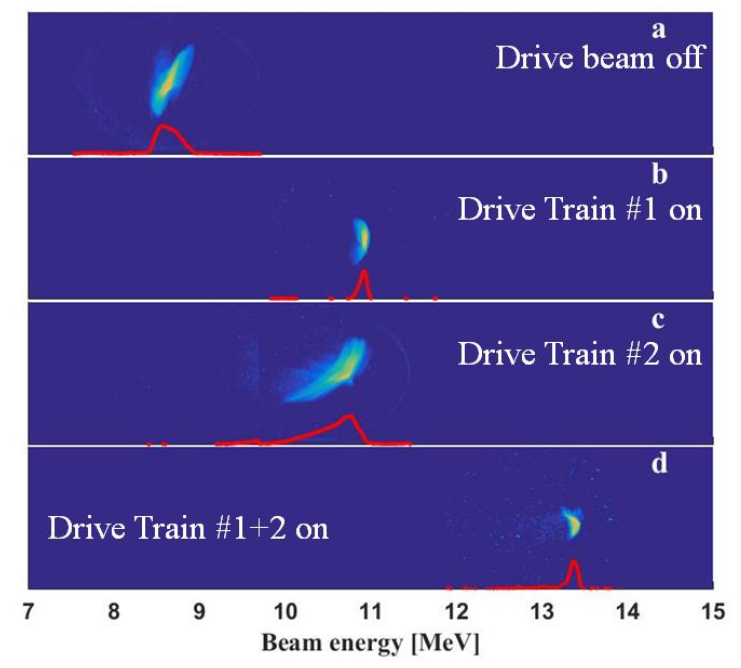
\includegraphics[width=0.75\textwidth]{images/old_tba}
	\label{fig:old-tba}
	\caption{Measurements of the energy during simplified staging experiments, 
		figure courtesy of Gwanghui Ha at AWA.
		Drive Train 1 refers to the stage one, and Drive Train 2 to stage 2. 
		Energy gain was observed in each stage independently.
		A larger energy gain was observed when both stages supplied RF to the witness beam line.}
\end{figure}
%%%%%%%%%%%%%%%%%%%%%%%%%%%%%%%%%%%%%%%%%%%%%%%%%%%%%%%%%%%%%%%%%%%%%%%%%%%%%%%%%%%%%%%%%%%%


%%%%%%%%%%%%%%%%%%%%%%%%%%%%%%%%%%%%%%%%%%%%%%%%%%%%%%%%%%%%%%%%%%%%%%%%%%%%%%%%
\Section{Simplified Staging Results}





\Section{AWA Design Requirements} \label{sec:requirements}

\lsnote{{\it Not sure if this section should be here, or later, more toward end of chapter.  This section is probably where you should have the overview of simple staging versus full staging, and a summary of what was required to go to full staging.  The title of the section should also be changed, maybe `Fully staged two beam acceleration'?  Probably need another (or repeated) figure here.}}
% An example for enumerate
\begin{enumerate}
        \item Kicker Design
        \item Septum Design
        \item Optimization
\end{enumerate}

% A quotation example
% Every quota must be accompanied by a reference to the source
% in a footnote or in the Bibliography
\begin{quotation}
        test
\end{quotation}

%%%%%%%%%%%%%%%%%%%%%%%%%%%%%%%%%%%%%%%%%%%%%%%%%%%%%%%%%%%%%%%%%%%%%%%%%%%%%%%%%%%%%%%%%%%%
%%%%%%%%%%%%%%%%%%%%%%%%%%%%%%%%%%%%%%%%%%%%%%%%%%%%%%%%%%%%%%%%%%%%%%%%%%%%%%%%%%%%%%%%%%%%
\Section{Fully Staged Two Beam Acceleration}

\lsnote{This is probably where you should have the overview of simple staging versus full staging, and a summary of what was required to go to full staging.  The title of the section should also be changed, maybe `Fully staged two beam acceleration'?}

In order to design and test the desired beam line, three technologies 
new to the AWA were investigated. These include a kicker, septum magnets, 
and non-GA optimization algorithms.

% An example for enumerate
\begin{enumerate}
	\item Kicker Design
	\item Septum Design
	\item Optimization 
\end{enumerate}

% A quotation example
% Every quota must be accompanied by a reference to the source
% in a footnote or in the Bibliography
\begin{quotation}
	test
\end{quotation}



\Section{Thesis Outline}

The rest of the thesis details work done at AWA.
Chapter 2 covers experimental measurements and preparations for TBA.
These include RF measurements and beam diagnostics (energy, beam size, and bunch length measurements).
Chapter 3 discusses simulation work done to model the drive line at AWA.
This includes optimization work.
Chapter 4 covers kicker and beam line optics design for fully staged TBA.

